\newpage
\section{Part III - Multi-variable control}
The objective of this chapter is to \textbf{control} the helicopter using a   multiple-input/multiple-output (MIMO) control system, to obtain a desirable behaviour of several output states by simultaneously manipulating multiple input channels.

\subsection{Problem 1 - Deriving a multi-varible controller}

We put the linerized equations \textbf{\tex(\ref{subeq1} - \ref{eq:Travel_ddot}})} into the (\ref{eq:multivariable}) state-space representation.


\begin{equation}
    \dot{\mathbf{x}} = \mathbf{Ax + Bu} } \label{eq:multivariable}
\end{equation}

We get the following state space system
\begin{equation} \label{eq:LQR}
      \begin{bmatrix}
        \dot{\tilde{p}} \\
        \ddot{\tilde{p}} \\
        \ddot{\tilde{e}}
    \end{bmatrix}
    =
    %A
     \begin{bmatrix}
    0 & 1 & 0 \\
    0 & 0 & 0 \\
    0 & 0 & 0 \\
    \end{bmatrix}
    %x
    \begin{bmatrix}
        \tilde{p} \\
        \dot{\tilde{p}} \\
        \dot{\tilde{e}}
    \end{bmatrix}
    + %second part
    %+B 
       \begin{bmatrix}
    0 & 0 \\
    0 & K_1 \\
    K_2 & 0 \\
    \end{bmatrix}
    %u
    \begin{bmatrix}
        \tilde{V}_s \\
        \tilde{V}_d
    \end{bmatrix}     
\end{equation}




\subsection{Problem 2- LQR}

Controlling the system using the LQR method, allows more flexibility when tuning the system, and is the preferred method for multi-input/multi-output (MIMO) systems.
The LQR control method places the poles of the system at the optimal place

The poles of the system are placed at the optimal place, by selecting on the weighing of matrices Q and R. In order to to do this the system must be controllable.

Controllability is a requirement that the output of the system can be steered to any desired position by manipulating the input. The state-space model in (\ref{eq:LQR}) is fully controllable if and only if the matrix C=
  \begin{bmatrix}
    B & AB & A^2B 
  \end{bmatrix} has full row rank. We test this in our matlab script and it is fully controllable, 
\newpage
\textbf{LQR MATLAB-script}
\begin{lstlisting}
LQR - Without Integral effect  
A_LQR = [0 1 0; 0 0 0; 0 0 0];
B_LQR = [0 0; 0 K1; K2 0];
C_LQR = [1 0 0; 0 0 1];
D_LQR = 0;

Rank_LQR = rank(ctrb(A_LQR,B_LQR)); %check if A Matrix is full rank

R_LQR = [1 0;0 1]; 
Q_LQR = 200*diag([2, %pitch
                  2/3, %pitch rate
                     3]); % elevation rate

[K_LQR,S_LQR,E_LQR]=lqr(A_LQR,B_LQR,Q_LQR,R_LQR); %Calculate the gain, and the eigenvalues
P_LQR = inv(C_LQR*inv(B_LQR*K_LQR-A_LQR)*B_LQR); 

\end{lstlisting}


A controller of the following form is desired
\begin{equation}
    \mathbf{u} = \mathbf{Pr - Kx}
\end{equation}
The matrix $\mathbf{K}$ corresponds to the linear quadratic regulator (LQR) for which the control input $\mathbf{u} = \mathbf{-Kx}$ optimizes the cost function
\begin{equation}
    J = \int_0^\infty \left( \mathbf{x}^T (t) \mathbf{Qx}(t) + \mathbf{u}^T (t) \mathbf{Ru} (t) \right) dt
\end{equation}
Bryson's rule was used as a starting point for finding reasonable matrices $\mathbf{Q}$ and $\mathbf{R}$. It states that they should be chosen to be diagonal with
\begin{subequations}
\begin{align}
    Q_{ii} &= \frac{1}{\text{maximum acceptable value of  } z_i^2} , \quad i \in {1, 2, \dots, l} \\
    R_{jj} &= \frac{1}{\text{maximum acceptable value of  } u_j^2} , \quad i \in {1, 2, \dots, k}
\end{align}
\end{subequations}

The chosen values is showed in the MATLAB script.

The choice of weighting matrices Q and R is a tradeoff between control performance (Q Large) and low input energy (R large), increasing both Q and R by the same factor leaves the optimal solution invariant. We tune the Q and R to the following:
\begin{equation}
    \mathbf{Q} =
    \begin{bmatrix}
        400 & 0 & 0 \\
        0 & 133.33 & 0 \\
        0 & 0 & 600
    \end{bmatrix}
    \quad \mathrm{and} \quad \mathbf{R} =
    \begin{bmatrix}
        1 & 0 \\
        0 & 1 \\
    \end{bmatrix}
\end{equation}
The corresponding matrix $\mathbf{K}$ was then obtained by using the MATLAB command {\fontfamily{qcr}\selectfont K=lqr(A,B,Q,R)}:
\begin{equation}
    \mathbf{K} = 
    \begin{bmatrix}
    0 & 0 & 24.49 \\
    20 & 14.3636 & 0
    \end{bmatrix}
\end{equation}


\textbf{Figure \ref{sim:2} and \ref{sim:3}}  show how the final system was setup in Simulink.

\begin{figure}[!htb]
 \centering
    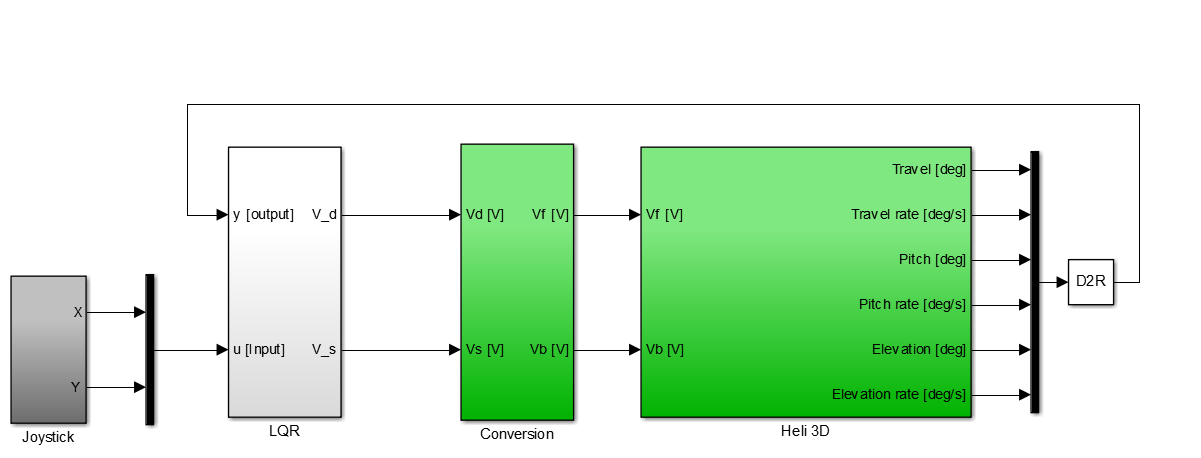
\includegraphics[scale=0.40]{images/LQR1}
       \caption{LQR with simulink}
    \label{sim:2}
\end{figure}




\begin{figure}[!htb]
 \centering
    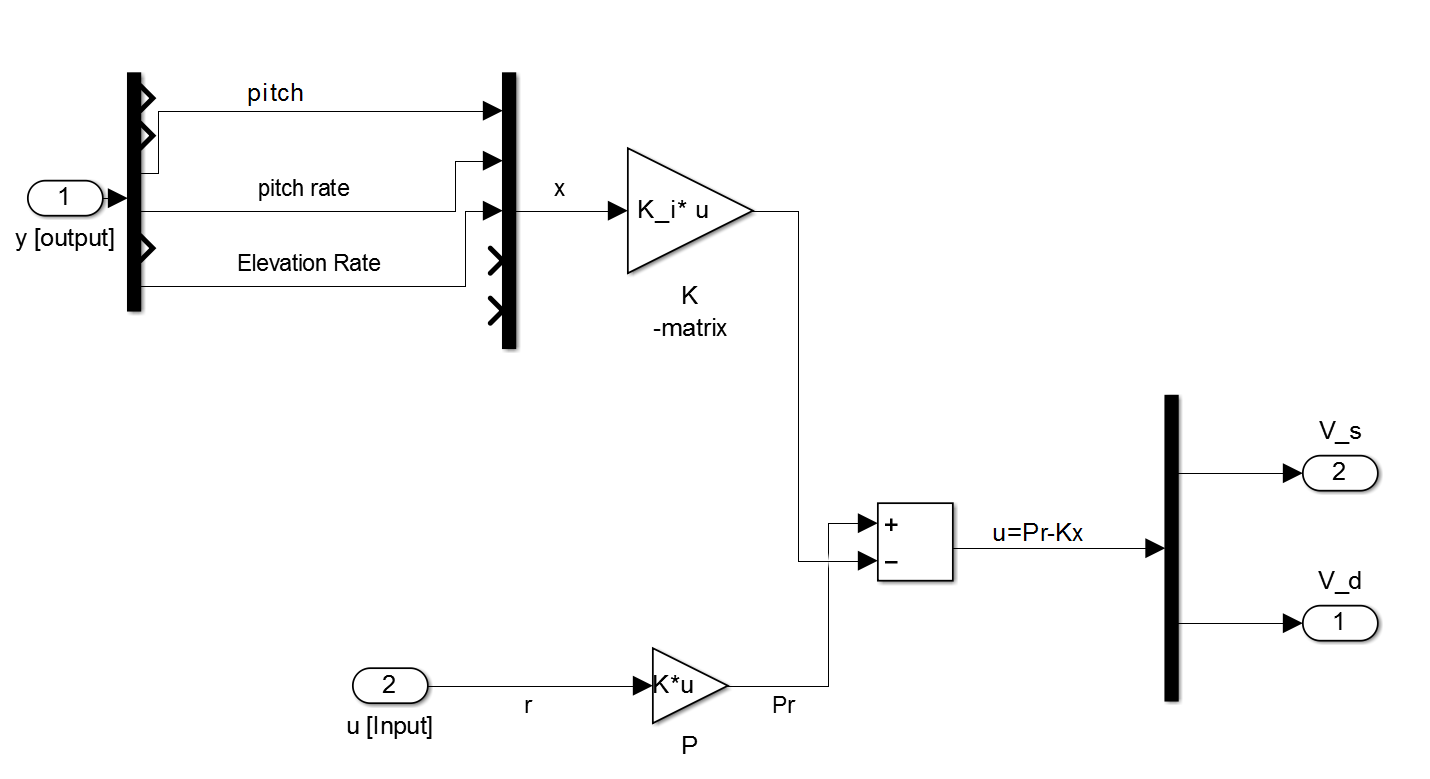
\includegraphics[scale=0.20]{images/LQR2}
       \caption{Inside LQR-Block}
    \label{sim:3}
\end{figure}









\newpage

\subsection{Problem 3 - Adding an integral effect }
Due to model imperfections, external disturbances and similar effects the controller
in its current form will not be able to reach a steady-state tracking error of zero. To account for this we can add an “integral” part. This is done by adding two new state variables:
\begin{equation}
\begin{split}
    \dot{\gamma} &= \tilde{p} - \tilde{p}_c \\
    \dot{\zeta} &= \dot{\tilde{e}} - \dot{\tilde{e}}_c
\end{split}
\end{equation}


The integral effect accounts for disturbances on the system. The output will tend towards a constant reference.

The new system is given by the following equation:
\begin{equation} \label{eq:LQR}
      \begin{bmatrix}
        \dot{\tilde{p}} \\
        \ddot{\tilde{p}} \\
        \ddot{\tilde{e}}\\
          \dot{\gamma} \\
        \dot{\zeta}
    \end{bmatrix}
    =
    %A
     \begin{bmatrix}
    0 & 1 & 0 & 0 & 0\\
    0 & 0 & 0 & 0 & 0 \\
    0 & 0 & 0 & 0 & 0 \\
    1 & 0 & 0 & 0 & 0 \\
    0 & 0 & 1 & 0 & 0
    \end{bmatrix}
    %x
    \begin{bmatrix}
        \tilde{p} \\
        \dot{\tilde{p}} \\
        \dot{\tilde{e}}\\
        \gamma\\
        \zeta
    \end{bmatrix}
    + %second part
    %+B 
       \begin{bmatrix}
    0 & 0 \\
    0 & K_1 \\
    K_2 & 0 \\
    0 & 0\\
    0 & 0
    \end{bmatrix}
    %u
    \begin{bmatrix}
        \tilde{V}_s \\
        \tilde{V}_d
    \end{bmatrix}     
\end{equation}


The system is tested for controllability and the weighing Q matrix is first tested with the Bryson's Rule start values, further a trial and error approached was used to find a satisfactory tuning. This is shown in the following MATLAB-Script


\textbf{LQR with integral    MATLAB-script}
\begin{lstlisting}
%Including Integral effect.
A_i = [0 1 0 0 0;0 0 0 0 0;0 0 0 0 0;1 0 0 0 0; 0 0 1 0 0];
B_i = [0 0;0 K1;K2 0; 0 0; 0 0];
C_i = [1 0 0 0 0;0 0 1 0 0];
D_i = 0;
Rank_i = rank(ctrb(A_i,B_i)); %check if A Matrix is full rank

R_i = diag([1,1]);
Q_bry = [(1/(pi/4)^2) 0 0;0 (1/(pi/16)^2) 0;0 0 1/(pi/16)^2];
Q_i = 100 . [[2.2 0 0 0 0];[0 0.8 0 0 0];[0 0 2 0 0];[0 0 0 1/20 0];[0 0 0 0 5]];

[K_i,S_i,E_i] = lqr(A_i,B_i,Q_i,R_i); %Find state feedback K gain vector
P_i = pinv(B_i)*(B_i*K_i-A_i)*pinv(C_i);
%P_i = K_i*C_i'; %another method 
\end{lstlisting}
      
      

The LQR-block is changed to add two 


\begin{figure}[!htb]
 \centering
    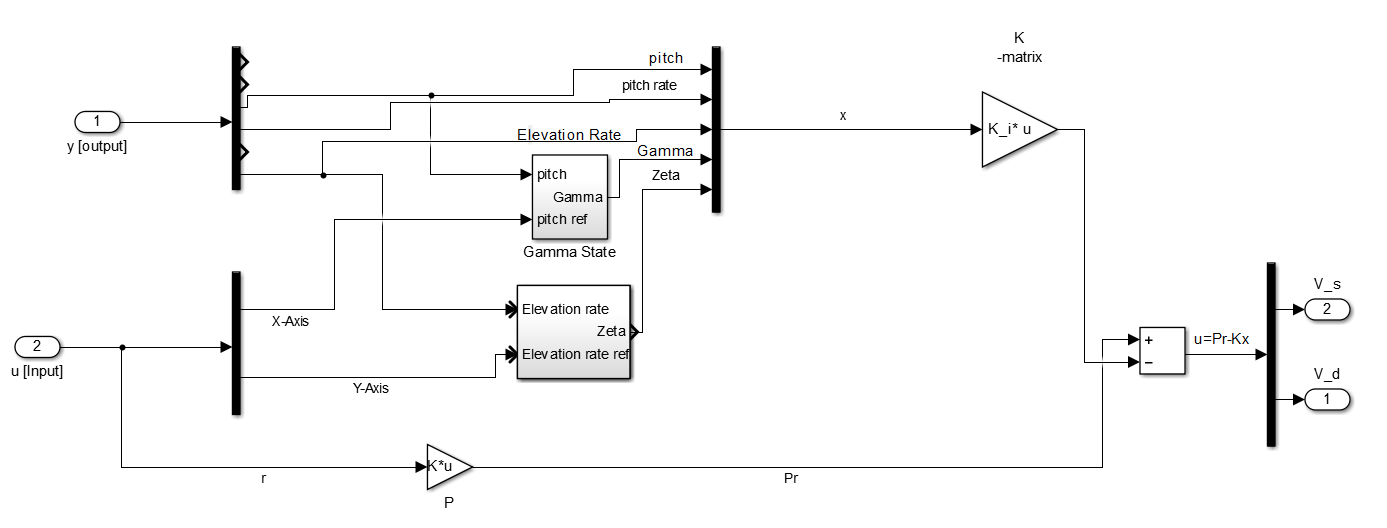
\includegraphics[scale=0.30]{images/LQR3}
       \caption{Inside LQR-Block with Integral}
    \label{sim:4}
\end{figure}



\begin{figure}[!htb]
 \centering
    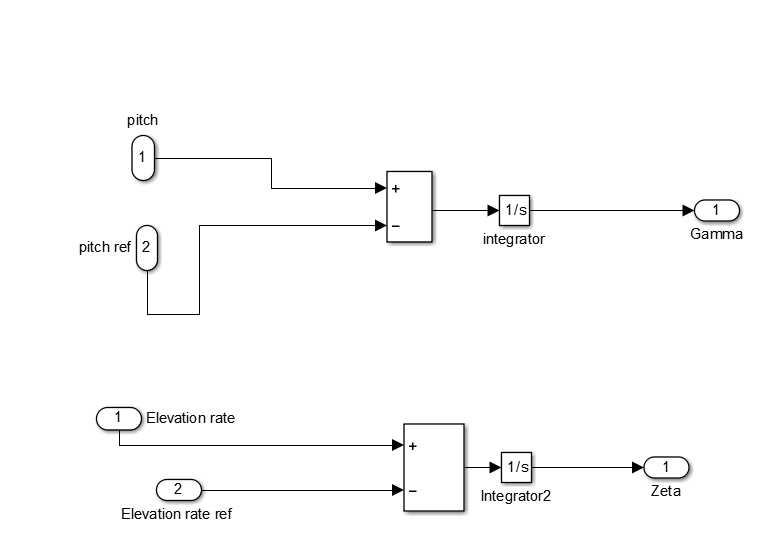
\includegraphics[scale=0.50]{images/LQR4}
       \caption{Inside Gamma and Zeta}
    \label{sim:5}
\end{figure}

